\documentclass{beamer}


\usetheme{PSY9511}

\title{Russell's Paradox}
\author{Esten H. Leonardsen}
\date{10.02.25}


\begin{document}
	\begin{frame}
	 	\maketitle
	\end{frame}

    \begin{frame}{Background}
        \begin{tikzpicture}
            \node[] at (-5.25, -3.5) {};
            \node[] at (5.25, 3.5) {};

            \visible<1-2>{
                \node[inner sep=0pt, draw=black, rotate=90] at (-2.675, 0) {
                    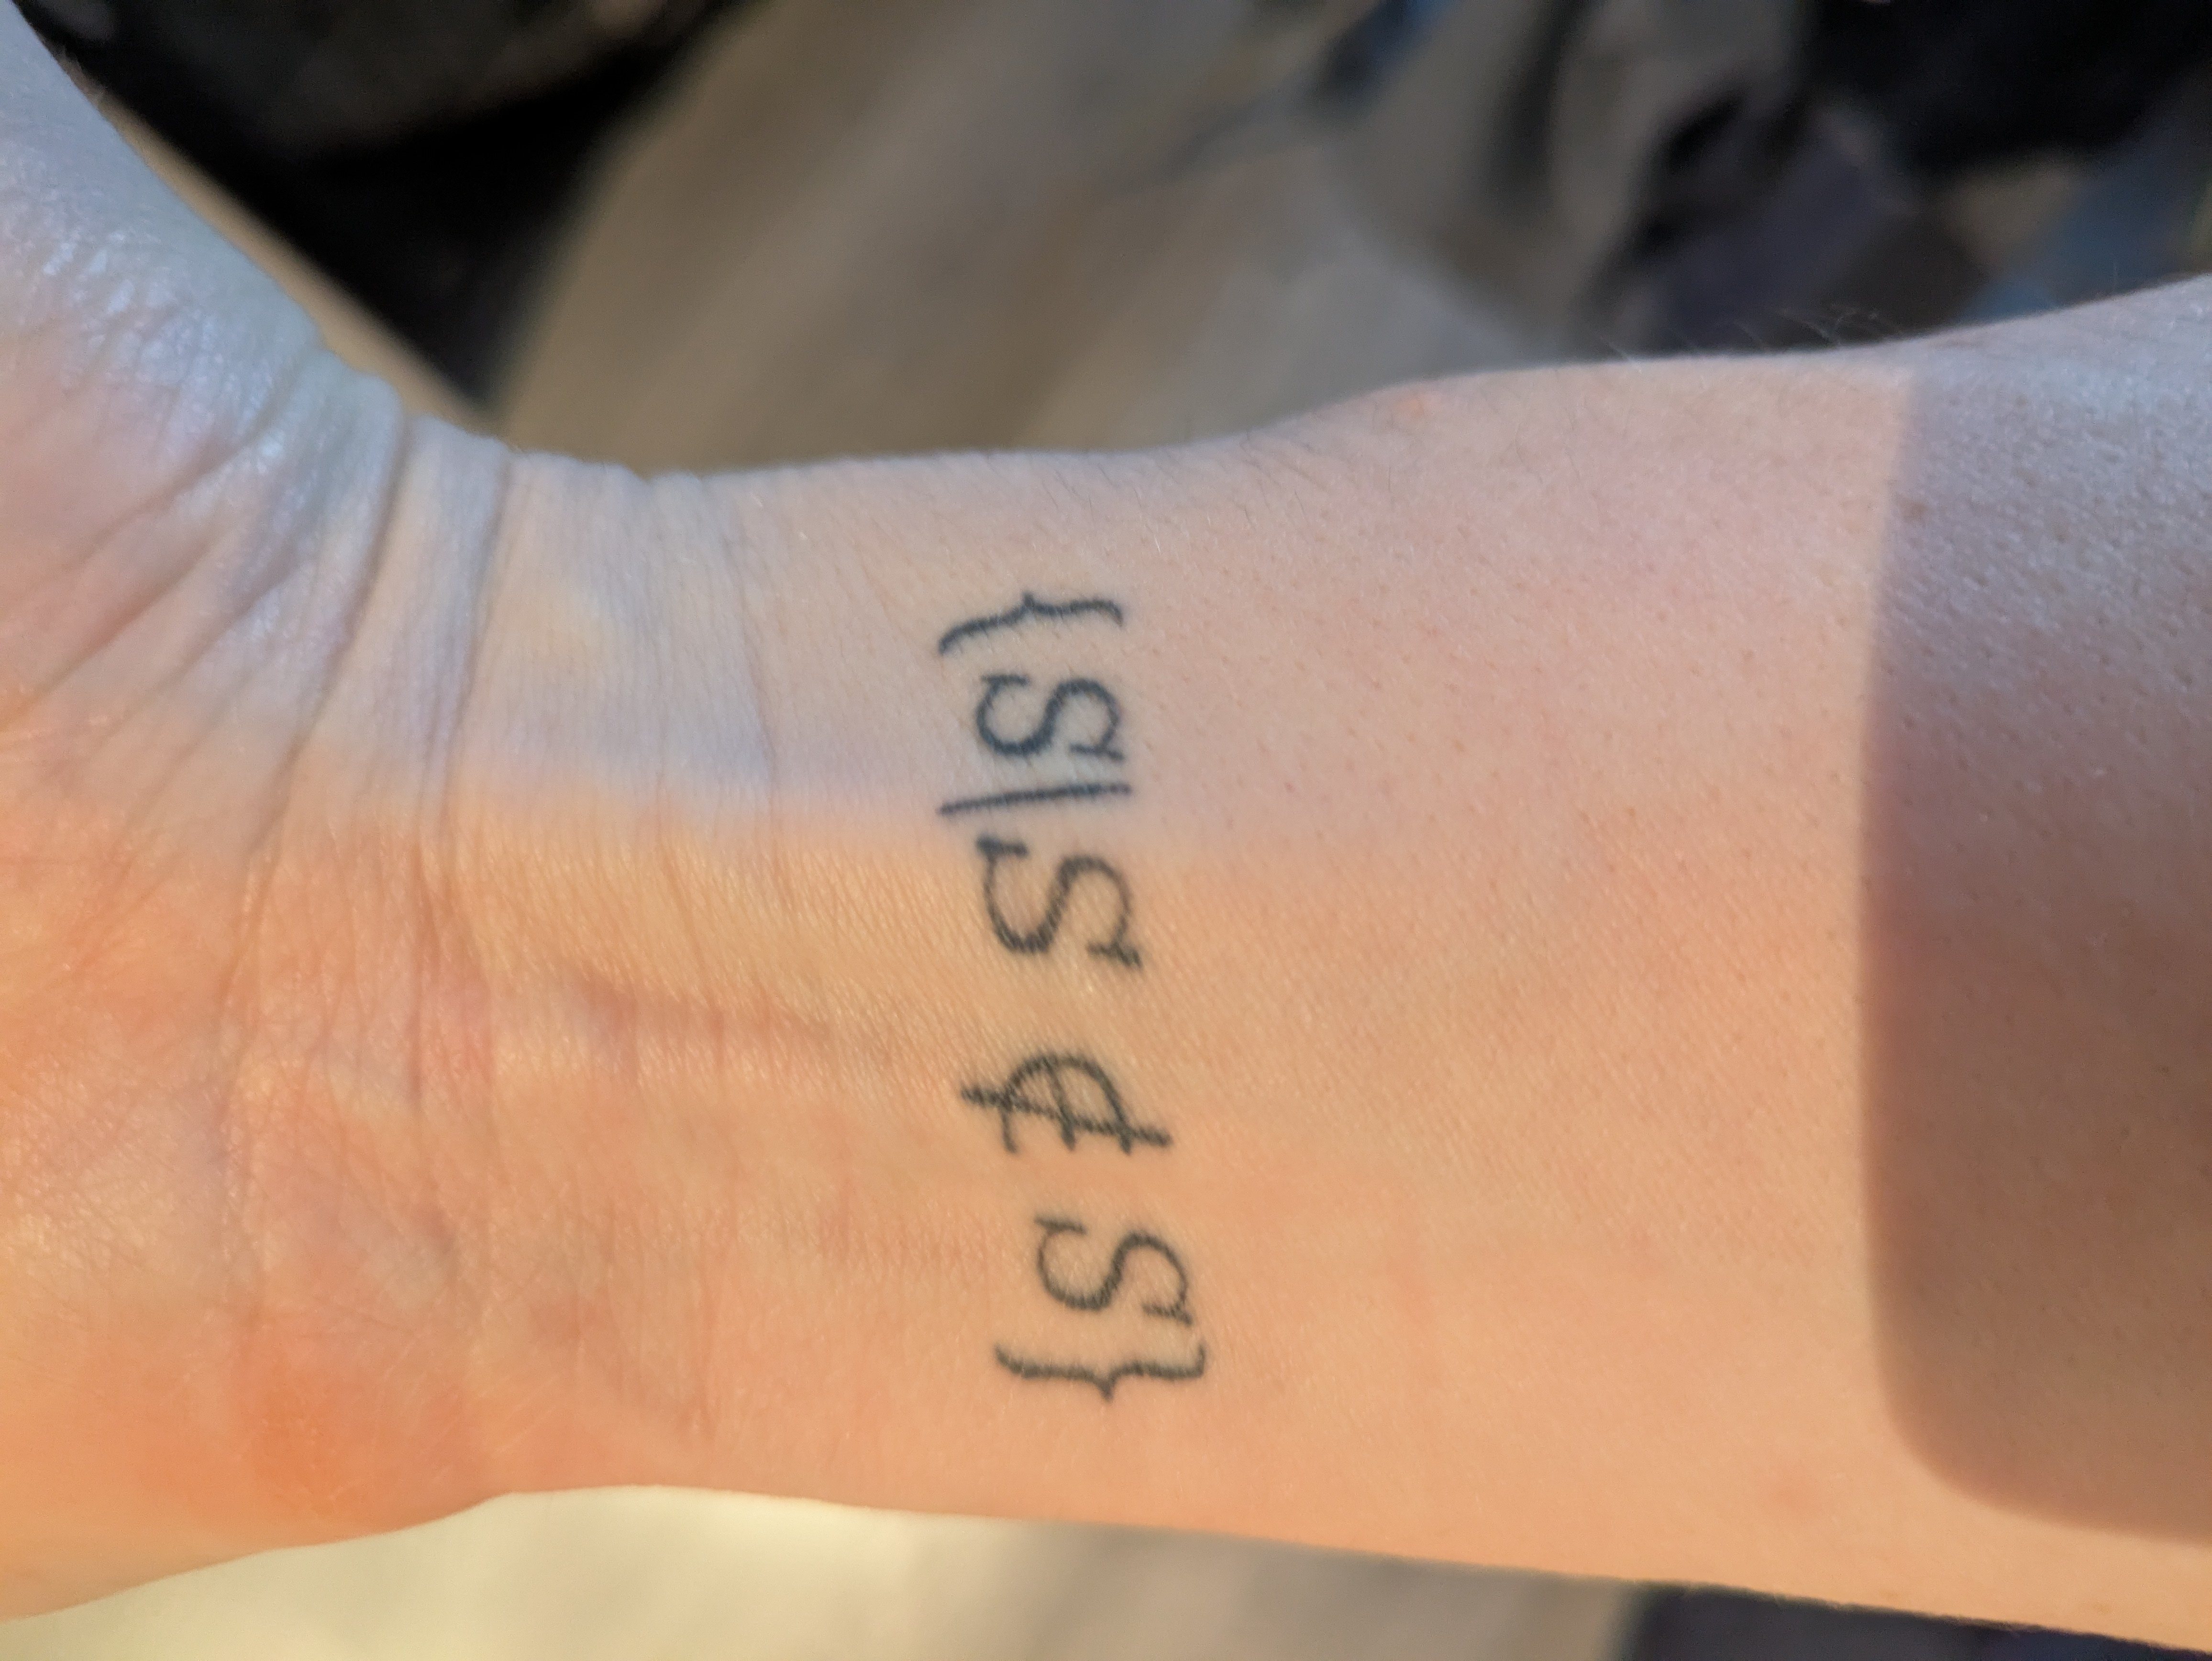
\includegraphics[width=5cm]{data/tattoo.jpg}
                };
            }
            \visible<2>{
                \node[] at (2.675, 0) {
                    $\{S | S \notin S\}$
                };
            }
            \visible<3>{
                \node[inner sep=0pt, draw=black, label=below:\tiny{Source: A guy I met at a party once}] at (0, 0) {
                    \includegraphics[width=9cm]{data/westworld.jpg}
                };
            }
        \end{tikzpicture}
    \end{frame}

    \begin{frame}{Historical underpinnings}
        \begin{tikzpicture}
            \node[draw=black] at (-5.25, -3.5) {};
            \node[draw=black] at (5.25, 3.5) {};

            \visible<1>{
                \node[inner sep=0pt, draw=black] at (0, 0) {
                    \includegraphics[width=4.5cm]{data/plato.JPG}
                };
            }
            \visible<2>{
                \node[inner sep=0pt, draw=black] at (0, 0) {
                    \includegraphics[width=7.5cm]{data/cave.jpg}
                };
            }
            \visible<3>{
                \node[inner sep=0pt, draw=black] at (0, 0) {
                    \includegraphics[width=6cm]{data/kant.jpeg}
                };
            }
            \visible<4-5>{
                \node[inner sep=0pt, draw=black] at (-2.675, 0) {
                    \includegraphics[height=5cm]{data/frege.jpg}
                };
            }
            \visible<5>{
                \node[inner sep=0pt, draw=black] at (2.675, 0) {
                    \includegraphics[height=5cm]{data/russell.jpg}
                };
            }
        \end{tikzpicture}
    \end{frame}

\end{document}
